\section{Programming [80 pts]}
\label{programming}

Your goal in this assignment is to implement a working Natural Language Processing (NLP) system, i.e., a sentiment polarity analyzer, using binary logistic regression. You will then use your algorithm to determine whether a review is positive or negative using movie reviews as data. You will do some very basic feature engineering, through which you are able to improve the learner's performance on this task. You will write two programs: \texttt{feature.\{py|java|cpp|m\}} and \texttt{lr.\{py|java|cpp|m\}} to jointly complete the task. The programs you write will be automatically graded using the Autolab system. You may write your programs in {\bf Octave, Python, Java,} or {\bf C++}. However, you should use the same language for all parts below.


\subsection{The Tasks and Data Sets}\label{dataset}


  {\bf Materials } Download the tar file from Autolab (``Download handout"). The tar file will contain all the data that you will need in order to complete this assignment.
  
 The handout contains data from the Movie Review Polarity data set (for more details, see \url{http://www.cs.cornell.edu/people/pabo/movie-review-data/}).  Currently, the original data is distributed as a collection of separate files (one movie review per file). In the Autolab handout, we have converted this to a one line per example format consisting of the label 0 or 1 in the first column followed by all the words in the movie review (with none of the line breaks) in the second column.
 
 
 
 Each data point consists of a label (0 for negatives and 1 for positives) and a attribute (a set of words as a whole). In the attribute, words are separated using white-space (punctuations are also separated with white-space). All characters are lowercased. No fancy pre-processing on the plain text is needed, because we have already done most of the work for you in the handout. We also provide a dictionary file (\lstinline{dict.txt}) to limit the vocabulary to be considered in this assignments. Actually, this dictionary is constructed from the training data. Examples of the dictionary content are as follows, where the second column is the index of the word. Column one and column two are separated with white-space. Each line in \lstinline{dict.txt}  has the format: \lstinline{word index\n}.
 
 \begin{lstlisting}
films 0
adapted 1
from 2
comic 3
\end{lstlisting}
 
 Examples of the data are as follows.
 
 
\begin{lstlisting}
1 david spade has a snide , sarcastic sense of humor that works ... 
0 " mission to mars " is one of those annoying movies where , in ...
1 anyone who saw alan rickman's finely-realized performances in ...
1 ingredients : man with amnesia who wakes up wanted for murder , ...
1 ingredients : lost parrot trying to get home , friends synopsis : ... 
1 note : some may consider portions of the following text to be ...
0 aspiring broadway composer robert ( aaron williams ) secretly ...
0 america's favorite homicidal plaything takes a wicked wife in " ...
\end{lstlisting}

We have provided you with two subsets of the movie review data set. Each data set is divided into a training, a validation, and a test data set.
%
The small data set (\lstinline{smalltrain_data.tsv}, \lstinline{smallvalid_data.tsv}, and \lstinline{smalltest_data.tsv}) can be used while debugging your code. We have included the reference output files for this data set after \textbf{30 training epochs} (see directory \lstinline{smalloutput/}). 
%
We have also included a larger data set (\lstinline{train_data.tsv}, \lstinline{valid_data.tsv}, \lstinline{test_data.tsv}) with reference outputs for this data set after \textbf{60 training epochs}  (see directory \lstinline{largeoutput/}) . This data set can be used to ensure that your code runs fast enough to pass the autograder tests. Your code should be able to perform 60-epoch training and finish  predictions through all of the data in around one minute for each of the models: one minute for Model 1 and one minute for Model 2.

The data files are in tab-separated-value (\lstinline{.tsv}) format. This is identical to a comma-separated-value (\lstinline{.csv}) format except that instead of separating columns with commas, we separate them with a tab character, \lstinline{\t}. Each row is ended by a Unix style line ending, \lstinline{\n}. The first column always contains the label and the second column the set of words:  \lstinline{label\tword1 word2 word3 ... wordN\n}.
 
\subsection{Model Definition}\label{modeldescript}
 
 Assume you are given a data set with $N$ training examples and $M$ features. We first write down the \emph{negative} conditional log-likelihood of the training data in terms of the design matrix $\Xv$, the labels $\yv$, and the parameter vector $\thetav$. This will be your objective function $J(\thetav)$ for gradient descent. 
%
(Recall that $i$th row of the design matrix $\Xv$ contains the features $\xv^{(i)}$ of the $i$th training example. The $i$th entry in the vector $\yv$ is the label $y^{(i)}$ of the $i$th training example.  Here we assume that each feature vector $\xv^{(i)}$ contains a bias \emph{feature}, e.g. $x_0^{(i)} = 1 \,\,\forall i \in \{1,\ldots,N\}$. As such, \textbf{the bias parameter is folded into our parameter vector $\thetav$.}


Taking $\x^{\left(i\right)}$ to be a $(K+1)$-dimensional vector where $x^{(i)}_0=1$, the likelihood $p\left(\y|\mathbf{X},\thetav\right)$ is:
\begin{align}
     p(\y |\mathbf{X},\thetav) &= \prod_{i = 1}^N p(y^{(i)} | \x^{(i)}, \thetav) = \prod_{i = 1}^N \left(\frac{e^{\thetav^T\x^{\left(i\right)}}}{1+e^{\thetav^T\x^{\left(i\right)}}}\right)^{y^{(i)}}\left(\frac{1}{1+e^{\thetav^T\x^{\left(i\right)}}}\right)^{\left(1-y^{(i)}\right)}\\
    &= \prod_{i=1}^N \frac{\left(e^{\thetav^T\x^{\left(i\right)}}\right)^{y^{(i)}}}{1+e^{\thetav^T\x^{\left(i\right)}}}
\end{align}
Hence, the negative conditional log-likelihood is:
\begin{align}
    J(\thetav)= -\log p\left(\y|\mathbf{X},\thetav\right) &= \sum_{i=1}^N  -y^{(i)}\left(\thetav^T\x^{\left(i\right)}\right)+\log\left(1+e^{\thetav^T\x^{\left(i\right)}}\right)
\end{align}


The partial derivative of the negative log-likelihood $J(\thetav)$ with respect to $\thetav_j \,, j\in\{0,...,M\}$ is:
\begin{align}
    \frac{\partial J(\thetav)}{\partial \thetav_j} &= -\sum_{i=1}^N \x_j^{\left(i\right)}\left[y^{(i)}-\frac{e^{\thetav^T\x^{\left(i\right)}}}{1+e^{\thetav^T\x^{\left(i\right)}}}\right]
\end{align}


The gradient descent update rule  for binary logistic regression for parameter element $\thetav_j$ is

\begin{align}
    \thetav_j \leftarrow \thetav_j - \eta \frac{\partial J(\thetav)}{\partial \thetav_j}
\end{align}


Then, the stochastic gradient descent update for  parameter element $\thetav_j$ using the $i$th datapoint $(\x^{(i)},y^{(i)})$ is:
\begin{align}
    \thetav_j \leftarrow \thetav_j + \eta \x_j^{\left(i\right)}\left[y^{(i)}-\frac{e^{\thetav^T\x^{\left(i\right)}}}{1+e^{\thetav^T\x^{\left(i\right)}}}\right]
\end{align}
 


\subsection{Implementation}

The implementation consists of two programs, a feature extraction program \texttt{feature.\{py|java|cpp|m\}} and a sentiment analyzer program \texttt{lr.\{py|java|cpp|m\}} using binary logistic regression. The programming pipeline is illustrated as follows.

\begin{figure}[H]
        \centering
        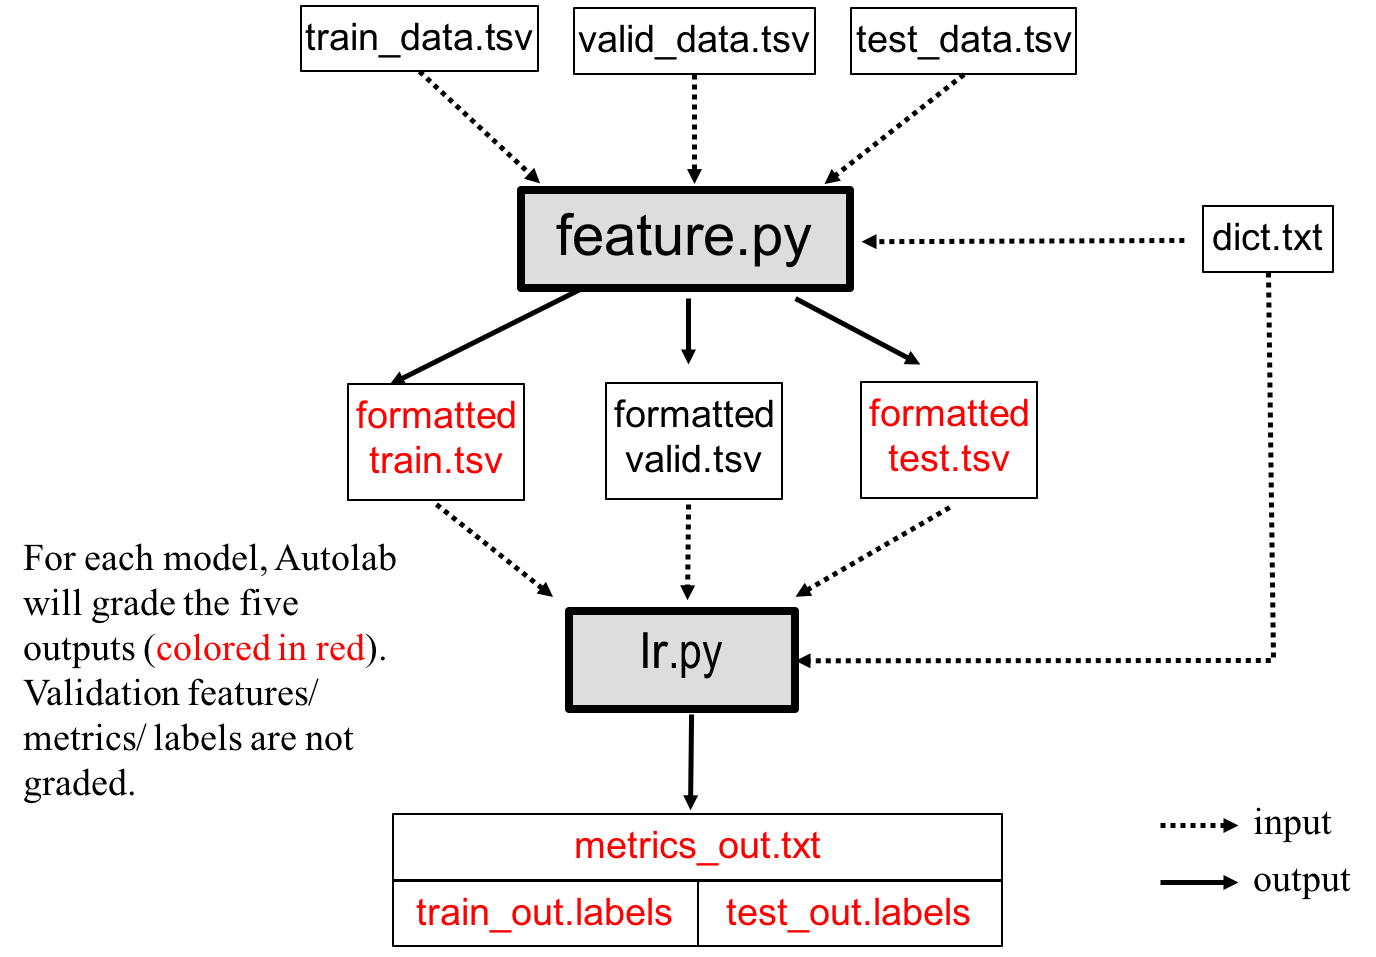
\includegraphics[width = 0.7\textwidth]{Pipeline.png}
        \caption{Programming pipeline for sentiment analyzer based on binary logistic regression}
        \label{pipeline}
\end{figure}


This first program is \texttt{feature.\{py|java|cpp|m\}}, that converts raw data (e.g., \lstinline{train_data.tsv}, \lstinline{valid_data.tsv}, and \lstinline{test_data.tsv}) into formatted training, validation and test data based on the vocabulary information in the dictionary file \lstinline{dict.txt}. To be specific, this program is to transfer the whole movie review text into a feature vector using some feature extraction methods. The formatted data sets should be stored in .tsv format. Details of formatted data sets will be introduced in Section~\ref{format_output} and Section~\ref{feature}.

The second program is \texttt{lr.\{py|java|cpp|m\}}, that implements a sentiment polarity analyzer using binary logistic regression. The file should learn the parameters of a binary logistic regression model that predicts a sentiment polarity (i.e. label) for the corresponding feature vector of each movie review. The program should output the labels of the training and test examples and calculate training and test error (percentage of incorrectly labeled reviews). As will be discussed later, efficient computation can be obtained with the help of the indexing information in the dictionary file \lstinline{dict.txt}.


Your implementation must satisfy the following requirements:
\begin{itemize}
    \item The \texttt{feature.\{py|java|cpp|m\}} must produce a sparse representation of the data using the label-index-value format \{\lstinline{label index[word1]:value1  index[word2]:value2...\n} \}. We will use unseen data to test your feature output separately. (see Section~\ref{format_output} and Section~\ref{feature} on feature engineering for details on how to do this). 
    \item Ignore the words not in the vocabulary of \lstinline{dict.txt} when the analyzer encounters one in the test or validation data.
    \item Set the trimming threshold to a constant $t=4$ for Model 2 feature extraction (see Section~\ref{feature}). 
    \item Initialize all model parameters to $0$.
    \item Use stochastic gradient descent (SGD) to optimize the parameters for a binary logistic regression model. The number of times SGD loops through all of the training data (\texttt{num\_epoch}) will be specified as a command line flag. Set your learning rate as a constant  $\eta = 0.1$.
    \item Perform stochastic gradient descent updates on the training data \textbf{in the order that the data is given in the input file}. Although you would typically shuffle training examples when using stochastic gradient descent, in order to autograde the assignment, we ask that you {\bf DO NOT} shuffle trials in this assignment.
    \item Be able to select which one of two feature extractions you will use in your logistic regression model using a command line flag (see Section~\ref{feature})
    \item Do not hard-code any aspects of the data sets into your code. We will autograde your programs on multiple (hidden) data sets that include different attributes and output labels.
\end{itemize}

Careful planning will help you to correctly and concisely implement your program. Here are a few \emph{hints} to get you started.
\begin{itemize}
    \item Write a function that takes a single SGD step on the $i$th training example. Such a function should take as input the model parameters, the learning rate, and the features and label for the $i$th training example. It should update the model parameters in place by taking one stochastic gradient step.
    \item Write a function that takes in a set of features, labels, and model parameters and then outputs the error (percentage of labels incorrectly predicted). You can also write a separate function that takes the same inputs and outputs the negative log-likelihood of the regression model.
\end{itemize}



\subsubsection{Command Line Arguments}
The autograder runs and evaluates the output from the files generated, using the following command (note \lstinline{feature} will be run before \lstinline{lr}):

\begin{tabbing}
For Python: \=\texttt{\$ \textbf{python} feature.\textbf{py} [args1\dots]}\\
\>\texttt{\$ \textbf{python} lr.\textbf{py} [args2\dots]}\\
For Java: \>\texttt{\$ \textbf{java} feature.\textbf{java} [args1\dots]}\\
\>\texttt{\$ \textbf{java} lr.\textbf{java} [args2\dots]}\\
For C++: \>\texttt{\$ \textbf{g++} feature.\textbf{cpp} ./a.out [args1\dots]}\\
\>\texttt{\$ \textbf{g++} lr.\textbf{cpp} ./a.out [args2\dots]}\\
For Octave: \>\texttt{\$ \textbf{octave} -qH feature.\textbf{m} [args1\dots]}\\
\>\texttt{\$ \textbf{octave} -qH lr.\textbf{m} [args2\dots]}
\end{tabbing}

Where above \texttt{[args1\dots]} is a placeholder for eight command-line arguments:\texttt{<train\_input>}\newline \texttt{<validation\_input> <test\_input> <dict\_input> <formatted\_train\_out> \newline <formatted\_validation\_out>  <formatted\_test\_out> <feature\_flag>}. These arguments are described in detail below:
\begin{enumerate}
    \item \texttt{<train\_input>}: path to the training input \texttt{.tsv} file (see Section~\ref{dataset})
    \item \texttt{<validation\_input>}: path to the validation input \texttt{.tsv} file (see Section~\ref{dataset})
    \item \texttt{<test\_input>}: path to the test input \texttt{.tsv} file (see Section~\ref{dataset})
    \item \texttt{<dict\_input>}: path to the dictionary input \texttt{.txt} file (see Section~\ref{dataset})
    \item \texttt{<formatted\_train\_out>}: path to output \texttt{.tsv} file to which the feature extractions on the \emph{training} data should be written (see Section~\ref{format_output})
    \item \texttt{<formatted\_validation\_out>}: path to output \texttt{.tsv} file to which the feature extractions on the \emph{validation} data should be written (see Section~\ref{format_output})
    \item \texttt{<formatted\_test\_out>}: path to output \texttt{.tsv} file to which the feature extractions on the \emph{test} data should be written (see Section~\ref{format_output})
    \item \texttt{<feature\_flag>}: integer taking value 1 or 2 that specifies whether to construct the Model 1 feature set or the Model 2 feature set (see Section~\ref{feature})---that is, if \lstinline{feature_flag}==1 use Model 1 features; if \lstinline{feature_flag}==2 use Model 2 features
\end{enumerate}


On the other hand, \texttt{[args2\dots]} is a placeholder for eight command-line arguments:\texttt{<formatted\_train\_input>}\newline \texttt{<formatted\_validation\_input> <formatted\_test\_input> <dict\_input> <train\_out> \newline <test\_out> <metrics\_out> <num\_epoch>}. These arguments are described in detail below:
\begin{enumerate}
    \item \texttt{<formatted\_train\_input>}: path to the formatted training input \texttt{.tsv} file (see Section~\ref{format_output})
    \item \texttt{<formatted\_validation\_input>}: path to the formatted validation input \texttt{.tsv} file (see Section~\ref{format_output})
    \item \texttt{<formatted\_test\_input>}: path to the formatted test input \texttt{.tsv} file (see Section~\ref{format_output})
    \item \texttt{<dict\_input>}: path to the dictionary input \texttt{.txt} file (see Section~\ref{dataset})
    \item \texttt{<train\_out>}: path to output \texttt{.labels} file to which the prediction on the \emph{training} data should be written (see Section~\ref{output})
    \item \texttt{<test\_out>}: path to output \texttt{.labels} file to which the prediction on the \emph{test} data should be written (see Section~\ref{output})
    \item \texttt{<metrics\_out>}: path of the output \texttt{.txt} file to which metrics such as train and test error should be written (see Section~\ref{metrics})
    %\item \texttt{<model\_out>}: path of the output \texttt{.txt} file to which the model parameters should be written (see Section~\ref{model})
    \item \texttt{<num\_epoch>}: integer specifying the number of times SGD loops through all of the training data (e.g., if \texttt{<num\_epoch>} equals 5, then each training example will be used in SGD 5 times). 
\end{enumerate}

As an example, if you implemented your program in Python, the following two command lines would run your programs on the data provided in the handout for 60 epochs using the features from Model 1.

\begin{lstlisting}[language=Shell]
$ python feature.py train_data.tsv valid_data.tsv test_data.tsv \
dict.txt formatted_train.tsv formatted_valid.tsv formatted_test.tsv 1

$ python lr.py formatted_train.tsv formatted_valid.tsv formatted_test\
.tsv dict.txt train_out.labels test_out.labels metrics_out.txt 60

\end{lstlisting}

\begin{notebox}
{\bf Important Note:} You will not be writing out the predictions on validation data, only on train and test data. The validation data is \emph{only} used to give you an estimate of held-out negative log-likelihood at the end of each epoch during training.\footnote{For this assignment, we will always specify the number of epochs. However, a more mature implementation would monitor the performance on validation data at the end of each epoch and stop SGD when this validation log-likelihood appears to have converged. You should \textbf{ \emph{not}} implement such a convergence check for this assignment.} 
\end{notebox}


\subsubsection{Output: Formatted Data Files} \label{format_output}
Your \lstinline{feature} program should write three output \texttt{.tsv} files converting original data to formatted data on \texttt{<formatted\_train\_out>}, \texttt{<formatted\_valid\_out>}, and \texttt{<formatted\_test\_out>}. Each should contain the formatted presentation for each example printed on a new line. Use \lstinline{\n} to create a new line. The format for each line should exactly match 

label\lstinline{\t}index[word1]:value1\lstinline{\t}index[word2]:value2\lstinline{\t}...index[wordM]:valueM\lstinline{\n}

Where above, the first column is label, and the rest are "index[word]:value" feature elements. index[word] is the index of the word in the dictionary, and value is the value of this feature (in this assignment, the value is one or zero). There is a colon, \lstinline{:}, between index[word] and corresponding value. Columns are separated using a table character, \lstinline{\t}. The handout contains example \texttt{<formatted\_train\_out>}, \newline \texttt{<formatted\_valid\_out>}, and \texttt{<formatted\_test\_out>} for your reference.

The formatted output will be checked separately by the autograder by running your \lstinline{feature} program on some unseen data sets and evaluating your output file against the reference formatted files. Examples of content of formatted output file are given below.

\begin{lstlisting}
0	2915:1	21514:1	166:1	32:1	10699:1	305:1	...
0	7723:1	51:1	8701:1	74:1	370:1	8:1    ...
1	229:1	48:1	326:1	43:1	576:1	55:1	...
1	8126:1	1349:1	58:1	4709:1	48:1	8319:1	...
\end{lstlisting}


\subsubsection{Output: Labels Files} \label{output}
Your \lstinline{lr} program should produce two output \texttt{.labels} files containing the predictions of your model on training data (\texttt{<train\_out>}) and test data (\texttt{<test\_out>}). Each should contain the predicted labels for each example printed on a new line. Use \lstinline{\n} to create a new line. 

Your labels should exactly match those of a reference implementation -- this will be checked by the autograder by running your program and evaluating your output file against the reference solution. Examples of the content of the output file are given below.

\begin{lstlisting}
0
0
1
0
\end{lstlisting}

\subsubsection{Output Metrics} \label{metrics}
Generate a file where you report the following metrics: 

\begin{description}

\item[error] After the final epoch (i.e. when training has completed fully), report the final training error \newline \lstinline{error(train)} and test error \lstinline{error(test)}. 
\end{description}

All of your reported numbers should be within 0.01 of the reference solution. The following is the reference solution for large data set with Model 1 feature structure after 60 training epochs. See \newline \lstinline{model1_metrics_out.txt} in the handout.

\begin{lstlisting}
error(train): 0.074167
error(test): 0.247500
\end{lstlisting}

Take care that your output has the exact same format as shown above. Each line should be terminated by a Unix line ending \lstinline{\n}. There is a whitespace character after the colon.



\subsubsection{Feature Engineering} \label{feature}

Your implementation of \texttt{feature.\{py|java|cpp|m\}} should have an input argument \texttt{<feature\_flag>} that specifies one of two types of feature extraction structures that should be used by the logistic regression model. The two structures are illustrated below as probabilities of the labels given the inputs.

\begin{description}
    \item[Model 1] $p(y^{(i)} \mid \bf{1}_{occur}( \x^{(i)},Vocab), \thetav)$: This model defines a probability distribution over the current label $y^{(i)}$ using the parameters $\thetav$ and a \emph{bag-of-word} feature vector $\bf{1}_{occur}( \x^{(i)},Vocab)$ indicating which word in vocabulary $\bf{Vocab}$ of the dictionary occurs at least once in the movie review example $\x^{(i)}$. The entry in the indicator vector associated  to the occurring word will set to one (otherwise, it is zero). This bag-of-word model should be used when \texttt{<feature\_flag>} is set to 1.
    
    \item[Model 2] $p(y^{(i)} \mid \bf{1}_{trim}(  \x^{(i)},Vocab,$ $t), \thetav)$: This model defines a probability distribution over the current label $y^{(i)}$ using the parameters $\thetav$ and a \emph{trimmed} bag-of-word feature vector $\bf{1}_{trim}( \x^{(i)},Vocab,$ $t)$ indicating  (1) which word in vocabulary $\bf{Vocab}$ of the dictionary occurs in the movie review example $\x^{(i)}$, AND (2) the \emph{count of the word} is LESS THAN ($<$) threshold $t$. The entry in the indicator vector associated  to the word that satisfies both conditions will set to one (otherwise, it is zero, including no shown and high-frequent words). This trimmed bag-of-word model should be used when \texttt{<feature\_flag>} is set to 2. In this assignment, use the constant trimming threshold $t=4$.
    
\end{description}

The motivation of Model 2 is that keywords that truly represent the sentiment may not occur too frequently, this trimming strategy can make the feature presentation cleaner by removing highly repetitive words that are useless and neutral, such "the", "a", "to", etc. You will observe whether this basic and heuristic strategy based on this intuition will bring in performance improvement.

Note that above $\bf{1}_{occur}$ and $\bf{1}_{trim}$ are described as a dense feature representation as showed in Tables \ref{tab:model1dense} for illustration purpose. In your implementation, you should further convert it to the representation in \ref{tab:model1sparse} for Model 1 and the representation in \ref{tab:model2sparse} for Model 2, such that the formatted data outputs match Section~\ref{format_output}.



\subsubsection{Evaluation}

Autolab will test your implementations on hidden data sets with the same format as the two data sets provided in the handout. \lstinline{feature} program and \lstinline{lr} program will be tested separately. To ensure that your code can pass the autolab tests in under 5 minutes (the maximum time length) be sure that your code can complete 60-epoch training and finish predictions through all of the data in the \lstinline{largedata} folder in around one minute for each of the models.

% Empirical Questions moved to problem1.tex (see Matt's note on Slack)

\subsection{Autolab Submission}

You must submit a .tar file named {\tt lr.tar} containing \texttt{feature.\{py|m|java|cpp\}} and \newline \texttt{lr.\{py|m|java|cpp\}}.
You can create that file by running:
\begin{lstlisting}
tar -cvf lr.tar feature.{py|m|java|cpp} lr.{py|m|java|cpp}
\end{lstlisting}
from the directory containing your code. 

Some additional tips: {\bf DO NOT} compress your files; you are just
creating a tarball. Do not use tar \texttt{-czvf}.  {\bf DO NOT} put
the above files in a folder and then tar the folder.  Autolab is case
sensitive, so observe that all your files should be named in {\bf
  lowercase}. You must submit this file to the corresponding homework
link on Autolab. The autograder for Autolab prints out some additional 
information about the tests that it ran. You can view this output by selecting 
 "Handin History" from the menu and then clicking one of the scores you 
 received for a submission. For example on this assignment, among other things, 
 the autograder will print out which language it detects (e.g. Python, Octave, C++, Java).  {\bf It is recommended that you create a new empty folder somewhere else, copy your implementation files there, and create tarball from there. This can ensure a clean submission without tarring unnecessary files.}
 
 \begin{notebox}
  {\bf Python3 Users:} Please include a blank file called python3.txt (case-sensitive) in your tar submission and we will execute your submitted program using Python 3 instead of Python 2.7.
 \end{notebox}

Note: For this assignment, you may make up to 10 submissions to Autolab before the deadline, but only your last submission will be graded.

    
    
    
%%%%%%%%%%%%%%%%%%%%%%%%%%%%%%%%%%%%%%%%%%%%%%%%%%%%%%%%%%%%%%%%%%%%%%%%%%%%%%%%%%%



